\documentclass[18pt,xcolor=table]{beamer}

%!TEX root = ./main.tex
\usepackage {bbm}
\usepackage {textpos}
\usepackage {tikz}
\usepackage {graphicx}


\definecolor{blue1}{RGB}{176,196,222 }
\definecolor{blue2}{RGB}{54,100,139}

\definecolor{grey1}{RGB}{139,139,131}
\definecolor{grey2}{RGB}{235,235,235}

\definecolor{black1}{RGB}{50,50,50}

\mode<presentation>
{
  % \usetheme{Pittsburgh}   
  %\usetheme{Boadilla}  
\usetheme{Madrid}  
  \usefonttheme[onlymath]{serif}
  \setbeamertemplate{items}[circle] 
  \setbeamertemplate{sections/subsections in toc}[circle]
  \setbeamercovered{invisible}
  \setbeamertemplate{navigation symbols}{}
% \usecolortheme{seahorse}
%
%  % Color Theme 
  \setbeamercolor{normal text}{bg=white,fg=black1} %All standard text
  \setbeamercolor{structure}{fg=blue2} %% Table of Contents 

  \setbeamercolor*{frametitle}{fg=black1,bg=grey2} % Frame title colors
%  \setbeamerfont{frametitle}{series=\bfseries}
  \setbeamercolor*{framesubtitle}{fg=blue2} % Frame subtitle color

  \setbeamercolor*{palette primary}{use=structure,fg=black1, bg=grey2} %right bottom
  \setbeamercolor*{palette secondary}{use=structure,bg=blue1} %middle bottom
  \setbeamercolor*{palette tertiary}{use=structure,bg=blue2,fg=grey2} %left bottom

  \setbeamercolor*{block body}{fg=black1,bg=blue1!10} % Color of blocks
  \setbeamercolor*{block title}{parent=structure,fg=black1,bg=blue1} % Block Titles
  \setbeamercolor{alerted text}{fg=blue2!85!black,} % Alerted Text (ie. highlight with \alert)
  \setbeamerfont{alerted text}{series=\bfseries}

  % not sure what these do.
  \setbeamercolor{item projected}{use=item,fg=black1,bg=item.fg!35}
  \setbeamercolor*{block title alerted}{parent=alerted text,bg=black1!15}
  \setbeamercolor*{block title example}{parent=example text,bg=black1!15}
  \setbeamerfont{framesubtitle}{size=\small}
}

\makeatletter
\setbeamertemplate{footline}
{
  \leavevmode%
    \hbox{%
      \begin{beamercolorbox}[wd=.333333\paperwidth,ht=2.25ex,dp=1ex,center]{author in head/foot}%
        \usebeamerfont{author in head/foot}\insertshortauthor%~~\beamer@ifempty{\insertshortinstitute}{}{(\insertshortinstitute)}
      \end{beamercolorbox}%
        \begin{beamercolorbox}[wd=.333333\paperwidth,ht=2.25ex,dp=1ex,center]{title in head/foot}%
        \usebeamerfont{title in head/foot}\insertshorttitle
        \end{beamercolorbox}%
        \begin{beamercolorbox}[wd=.333333\paperwidth,ht=2.25ex,dp=1ex,right]{date in head/foot}%
        \usebeamerfont{date in head/foot}\insertshortdate{}\hspace*{2em}
        \insertframenumber{} / \inserttotalframenumber\hspace*{2ex} 
      \end{beamercolorbox}}%
        \vskip0pt%
}
\makeatother

%\usepackage{kerkis}
\usepackage{helvet} 
\usepackage[T1]{fontenc}
\usepackage[protrusion=true,expansion=true]{microtype}
\usepackage{amsmath}

\renewcommand*{\thefootnote}{\fnsymbol{footnote}}


\pgfdeclareimage[height=1.5cm]{logo}{./logos/hd_logo}
\pgfdeclareimage[height=0.8cm]{small_logo}{./logos/hd_logo}

\AtBeginSection[] { 
  \begin{frame}[plain] 
    \frametitle{\bf Outline:}
    \framesubtitle{~~} 
    \tableofcontents[currentsection] 
  \end{frame} 
  \addtocounter{framenumber}{-1} 
} 

\setbeamercovered{transparent}

%%%%%%%%%%%%%%%%%%%%%%%
% user-defined commands
%%%%%%%%%%%%%%%%%%%%%%%
%!TEX root = ../main.tex


\newcommand{\beq}{\begin{equation}}
\newcommand{\eeq}{\end{equation}}

\newcommand{\eq}[1]{\begin{align*}#1\end{align*}}

\newcommand{\bfi}{\begin{figure}}
\newcommand{\efi}{\end{figure}}

\newcommand{\icg}{\includegraphics}

\newcommand{\bdm}{\begin{displaymath}}
\newcommand{\edm}{\end{displaymath}}

\newcommand{\beqa}{\begin{eqnarray}}
\newcommand{\eeqa}{\end{eqnarray}}

\newcommand{\beqas}{\begin{eqnarray*}}
\newcommand{\eeqas}{\end{eqnarray*}}

\newcommand{\barr}{\begin{array}}
\newcommand{\earr}{\end{array}}

\newcommand{\bit}{\begin{itemize}}
\newcommand{\eit}{\end{itemize}}

\newcommand{\qq}[1]{\qquad \mbox{#1} \qquad}

\def\hyph{-\penalty0\hskip0pt\relax}

% Tikz
\definecolor{blue1}{RGB}{176,196,222 }
\definecolor{blue2}{RGB}{54,100,139}
\definecolor{grey1}{RGB}{139,139,131}
\definecolor{grey2}{RGB}{235,235,235}
\definecolor{black1}{RGB}{50,50,50}


%Spaces
\newcommand{\Sp}[1]{{\cal #1}}
%
\newcommand{\sA}{\Sp{A}}
\newcommand{\sB}{\Sp{B}}
\newcommand{\sC}{\Sp{C}}
\newcommand{\sD}{\Sp{D}}
\newcommand{\sE}{\Sp{E}}
\newcommand{\sF}{\Sp{F}}
\newcommand{\sG}{\Sp{G}}
\newcommand{\sH}{\Sp{H}}
\newcommand{\sI}{\Sp{I}}
\newcommand{\sJ}{\Sp{J}}
\newcommand{\sK}{\Sp{K}}
\newcommand{\sL}{\Sp{L}}
\newcommand{\sM}{\Sp{M}}
\newcommand{\sN}{\Sp{N}}
\newcommand{\sO}{\Sp{O}}
\newcommand{\sP}{\Sp{P}}
\newcommand{\sQ}{\Sp{Q}}
\newcommand{\sR}{\Sp{R}}
\newcommand{\sS}{\Sp{S}}
\newcommand{\sT}{\Sp{T}}
\newcommand{\sU}{\Sp{U}}
\newcommand{\sV}{\Sp{V}}
\newcommand{\sW}{\Sp{W}}
\newcommand{\sX}{\Sp{X}}
\newcommand{\sY}{\Sp{Y}}
\newcommand{\sZ}{\Sp{Z}}

%Vectors
\newcommand{\V}[1]{{\bf #1}}
%
\newcommand{\va}{\V{a}}
\newcommand{\vb}{\V{b}}
\newcommand{\vc}{\V{c}}
\newcommand{\vd}{\V{d}}
\newcommand{\ve}{\V{e}}
\newcommand{\vf}{\V{f}}
\newcommand{\vg}{\V{g}}
\newcommand{\vh}{\V{h}}
\newcommand{\vi}{\V{i}}
\newcommand{\vj}{\V{j}}
\newcommand{\vk}{\V{k}}
\newcommand{\vl}{\V{l}}
\newcommand{\vm}{\V{m}}
\newcommand{\vn}{\V{n}}
\newcommand{\vo}{\V{o}}
\newcommand{\vp}{\V{p}}
\newcommand{\vq}{\V{q}}
\newcommand{\vr}{\V{r}}
\newcommand{\vs}{\V{s}}
\newcommand{\vt}{\V{t}}
\newcommand{\vu}{\V{u}}
\newcommand{\vv}{\V{v}}
\newcommand{\vw}{\V{w}}
\newcommand{\vx}{\V{x}}
\newcommand{\vy}{\V{y}}
\newcommand{\vz}{\V{z}}

\newcommand{\vA}{\V{A}}
\newcommand{\vB}{\V{B}}
\newcommand{\vC}{\V{C}}
\newcommand{\vD}{\V{D}}
\newcommand{\vE}{\V{E}}
\newcommand{\vF}{\V{F}}
\newcommand{\vG}{\V{G}}
\newcommand{\vH}{\V{H}}
\newcommand{\vI}{\V{I}}
\newcommand{\vJ}{\V{J}}
\newcommand{\vK}{\V{K}}
\newcommand{\vL}{\V{L}}
\newcommand{\vM}{\V{M}}
\newcommand{\vN}{\V{N}}
\newcommand{\vO}{\V{O}}
\newcommand{\vP}{\V{P}}
\newcommand{\vQ}{\V{Q}}
\newcommand{\vR}{\V{R}}
\newcommand{\vS}{\V{S}}
\newcommand{\vT}{\V{T}}
\newcommand{\vU}{\V{U}}
\newcommand{\vV}{\V{V}}
\newcommand{\vW}{\V{W}}
\newcommand{\vX}{\V{X}}
\newcommand{\vY}{\V{Y}}
\newcommand{\vZ}{\V{Z}}

\newcommand{\vone}{\V{1}}
\newcommand{\vzero}{\V{0}}
\newcommand{\B}{\V{B}}
\newcommand{\E}{\V{E}}
\newcommand{\Er}{\V{E}_r}
\newcommand{\Es}{\V{E}_s}
\newcommand{\un}{\hat{\vn}}



%Vectors
\newcommand{\T}[1]{\underline{\bf #1}}
%
\newcommand{\ta}{\T{a}}
\newcommand{\tb}{\T{b}}
\newcommand{\tc}{\T{c}}
%\newcommand{\td}{\T{d}}
\newcommand{\te}{\T{e}}
\newcommand{\tf}{\T{f}}
\newcommand{\tg}{\T{g}}
%\newcommand{\th}{\T{h}}
\newcommand{\ti}{\T{i}}
\newcommand{\tj}{\T{j}}
\newcommand{\tk}{\T{k}}
\newcommand{\tl}{\T{l}}
\newcommand{\tm}{\T{m}}
\newcommand{\tn}{\T{n}}
%\newcommand{\to}{\T{o}}
\newcommand{\tp}{\T{p}}
\newcommand{\tq}{\T{q}}
\newcommand{\tr}{\T{r}}
\newcommand{\ts}{\T{s}}
%\newcommand{\tt}{\T{t}}
\newcommand{\tu}{\T{u}}
\newcommand{\tv}{\T{v}}
\newcommand{\tw}{\T{w}}
\newcommand{\tx}{\T{x}}
\newcommand{\ty}{\T{y}}
\newcommand{\tz}{\T{z}}

\newcommand{\tA}{\T{A}}
\newcommand{\tB}{\T{B}}
\newcommand{\tC}{\T{C}}
\newcommand{\tD}{\T{D}}
\newcommand{\tE}{\T{E}}
\newcommand{\tF}{\T{F}}
\newcommand{\tG}{\T{G}}
\newcommand{\tH}{\T{H}}
\newcommand{\tI}{\T{I}}
\newcommand{\tJ}{\T{J}}
\newcommand{\tK}{\T{K}}
\newcommand{\tL}{\T{L}}
\newcommand{\tM}{\T{M}}
\newcommand{\tN}{\T{N}}
\newcommand{\tO}{\T{O}}
\newcommand{\tP}{\T{P}}
\newcommand{\tQ}{\T{Q}}
\newcommand{\tR}{\T{R}}
\newcommand{\tS}{\T{S}}
\newcommand{\tT}{\T{T}}
\newcommand{\tU}{\T{U}}
\newcommand{\tV}{\T{V}}
\newcommand{\tW}{\T{W}}
\newcommand{\tX}{\T{X}}
\newcommand{\tY}{\T{Y}}
\newcommand{\tZ}{\T{Z}}

\newcommand{\tone}{\T{1}}
\newcommand{\tzero}{\T{0}}

%Matrix
\newcommand{\M}[1]{{\mathbb #1}}
%
\newcommand{\mA}{\M{A}}
\newcommand{\mB}{\M{B}}
\newcommand{\mC}{\M{C}}
\newcommand{\mD}{\M{D}}
\newcommand{\mE}{\M{E}}
\newcommand{\mF}{\M{F}}
\newcommand{\mG}{\M{G}}
\newcommand{\mH}{\M{H}}
\newcommand{\mI}{\M{I}}
\newcommand{\mJ}{\M{J}}
\newcommand{\mK}{\M{K}}
\newcommand{\mL}{\M{L}}
\newcommand{\mM}{\M{M}}
\newcommand{\mN}{\M{N}}
\newcommand{\mO}{\M{O}}
\newcommand{\mP}{\M{P}}
\newcommand{\mQ}{\M{Q}}
\newcommand{\mR}{\M{R}}
\newcommand{\mS}{\M{S}}
\newcommand{\mT}{\M{T}}
\newcommand{\mU}{\M{U}}
\newcommand{\mV}{\M{V}}
\newcommand{\mW}{\M{W}}
\newcommand{\mX}{\M{X}}
\newcommand{\mY}{\M{Y}}
\newcommand{\mZ}{\M{Z}}

\newcommand{\mzero}{\M{0}}
\newcommand{\mone}{\M{1}}

% Derivatives
\newcommand{\pd}[2]{\frac{\partial #1}{\partial #2}}
\newcommand{\ppd}[2]{\frac{\partial^2 #1}{\partial #2^2}}
\newcommand{\td}[2]{\frac{\mathrm{d} #1}{\mathrm{d} #2}}

\newcommand{\px}{ \partial_{x} }
\newcommand{\py}{ \partial_{y} }
\newcommand{\pz}{ \partial_{z} }
\newcommand{\pt}{ \partial_{t} }
\newcommand{\ptt}{ \partial_{tt} }

\newcommand{\Div}[1]{\nabla \cdot #1}
\newcommand{\Curl}[1]{\nabla \times #1}
\newcommand{\Ctwo}[1]{\nabla_2 \times #1}
\newcommand{\Grad}[1]{\nabla #1}
\newcommand{\Gperp}[1]{\nabla^\perp #1}
\newcommand{\Lap}[1]{\Delta #1}

%integral d
\newcommand{\dd}[0]{\, \mathrm{d}}

% common discrete quantities
\newcommand{\dt}[0]{\delta t}

% physical variables
\newcommand{\eps}[0]{\epsilon_0}
\newcommand{\mus}[0]{\mu_0}
\newcommand{\boltz}[0]{\kappa_B}
\newcommand{\s}[0]{\alpha}
\newcommand{\vths}[0]{v_{th_\s}}
\newcommand{\vthe}[0]{v_{th_e}}
\newcommand{\vthi}[0]{v_{th_i}}
\newcommand{\Om}[0]{\Omega}
\newcommand{\bdOm}{\partial \Omega}

% bracketing
\newcommand{\inner}[2]{\langle #1, #2 \rangle}
\newcommand{\lb}[0]{\left[}
\newcommand{\rb}[0]{\right]}
\newcommand{\parn}[1]{\left( #1 \right)}
\newcommand{\la}{\langle}
\newcommand{\ra}{\rangle}
\newcommand{\lcb}{\left\{}
\newcommand{\rcb}{\right\}}

\newcommand{\mathAnd}{\,\,\mbox{and}\,\,}
\newcommand{\mathOn}{\,\,\mbox{on}\,\,}

\newcommand{\h}{\hat}
\newcommand{\wh}{\widehat}
%\newcommand{\ul}{\underline}

% math operators
\DeclareMathOperator{\Trace}{trace}
\DeclareMathOperator{\Supp}{supp}
\DeclareMathOperator{\Span}{span}
\DeclareMathOperator{\floor}{floor}
\DeclareMathOperator{\diam}{diam}
\DeclareMathOperator{\ceil}{ceil}
\DeclareMathOperator*{\argmin}{arg\,min}


\newcommand{\red}[1]{\textcolor{red}{#1}}
%added macro definitions here

\usepackage{tikz}
\usepackage{tabularx}
\usetikzlibrary{decorations.markings}
\usetikzlibrary{arrows,positioning} 

\usepackage{cancel}
\usepackage{hyperref}
\usepackage{caption}
\usepackage{subcaption}
\usepackage[]{algorithm}
\usepackage{algpseudocode}
\captionsetup{compatibility=false}


\title[Multigrid]{Introduction to Multigrid Methods}
\subtitle{Day 2: Geometric Multigrid}
\author[Mitchell]{Wayne Mitchell}
\institute{\pgfuseimage{logo}\\Universit\"at Heidelberg\\Institut f\"ur Technische Informatik}
\date[]{\alert{}}


\begin{document}
%!TEX root = ./main.tex
\tikzstyle{block} = [rectangle, draw, rounded corners, shade, top color=white, text width=5em,
  bottom color=blue!50!black!20, draw=blue!40!black!60, very thick, text centered, minimum height=4em]
  \tikzstyle{line} = [draw, -latex']
  \tikzstyle{cloud} = [draw, ellipse,top color=white, bottom color=red!20, node distance=2cm, minimum height=2em]

  \frame{\titlepage}

  \addtobeamertemplate{frametitle}{}{%
      \begin{textblock*}{100mm}(0.9\textwidth,-0.88cm)
    \pgfuseimage{small_logo}
    \end{textblock*}
  }

\AtBeginSection[] { 
  \begin{frame}[t]
    \frametitle{\bf Outline:}
    \framesubtitle{~~} 
    \tableofcontents[currentsection] 
  \end{frame} 
  \addtocounter{framenumber}{-1} 
} 

\let\tempone\itemize
\let\temptwo\enditemize
\renewenvironment{itemize}{\tempone\addtolength{\itemsep}{0.5\baselineskip}}{\temptwo}

\DeclareRobustCommand{\Chi}{\raisebox{2pt}{$\chi$}}
%%%%%%%%%%%%%%%%%%%%%%%%%%%%%%%%%%%%%%%%%%%%%%%%%%%%%%%%%%%%%%%%%%%%%%%%%%%%%%%%

\begin{frame}
\frametitle{\bf Outline:}
\framesubtitle{~~}
\tableofcontents
\end{frame}

%%%%%%%%%%%%%%%%%%%%%%%%%%%%%%%%%%%%%%%%%%%%%%%%%%%%%%%%%%%%%%%%%%%%%%%%%%%%%%%%

\section{Introduction}

% Slide
\begin{frame}{Introduction}
\begin{block}{Day 2 Goals}
\bit
\item Basic theoretical motivations for multigrid
\item Define the basic components of multigrid: relaxation, interpolation, and restriction
\item Outline geometric multigrid on a model problem
\eit
\end{block}
\end{frame}

% Slide
\begin{frame}
\begin{block}{Acknowledgements}
\bit
\item These slides are based on previous tutorials by Steve McCormick, Van Henson, Rob Falgout, Irad Yavneh, David Moulton.
\item https://github.com/copper-multigrid-conference
\eit
\end{block}
\end{frame}

% Slide
\begin{frame}{Introduction}
\begin{block}{Resources}
\bit
\item A Multigrid Tutorial. Briggs, Henson, McCormick.
\item Multigrid. Trottenberg, Oosterlee, Sch\"uller.
\item Matrix Computations. Golub, Van Loan.
\eit
\end{block}
\end{frame}

%%%%%%%%%%%%%%%%%%%%%%%%%%%%%%%%%%%%%%%%%%%%%%%%%%%%%%%%%%%%%%%%%%%%%%%%%%%%%%%%

\section{Basic iterative methods on a model problem}


% Slide
\begin{frame}{Basic iterative methods on a model problem}
\begin{block}{Moving from basic iterative methods to multigrid}
\bit
\item Focus on a model elliptic PDE problem
\item Examine the behavior of basic iterative methods on this problem
\item Use that behavior to motivate the move towards multigrid
\eit
\end{block}
\end{frame}

% Slide
\begin{frame}{Basic iterative methods on a model problem}
\begin{block}{Model problem: Poisson}
\bit
\item Classic model problem is a simple Poisson problem with zero Dirichlet boundary conditions:
\eq{
\Delta u &= f, & \Omega \\
u &= 0, & \partial \Omega
}
\item Discretizing with finite differences on a regular 1D mesh:
\eit
\eq{
&\frac{-u_{i-1} + 2u_i - u_{i+1}}{h^2} = f_i, & i = 1,2,..., N-1 \\
&u_0 = u_N = 0
}
\end{block}
\end{frame}

% Slide
\begin{frame}{Basic iterative methods on a model problem}
\begin{block}{Model problem: Poisson}
\begin{center}
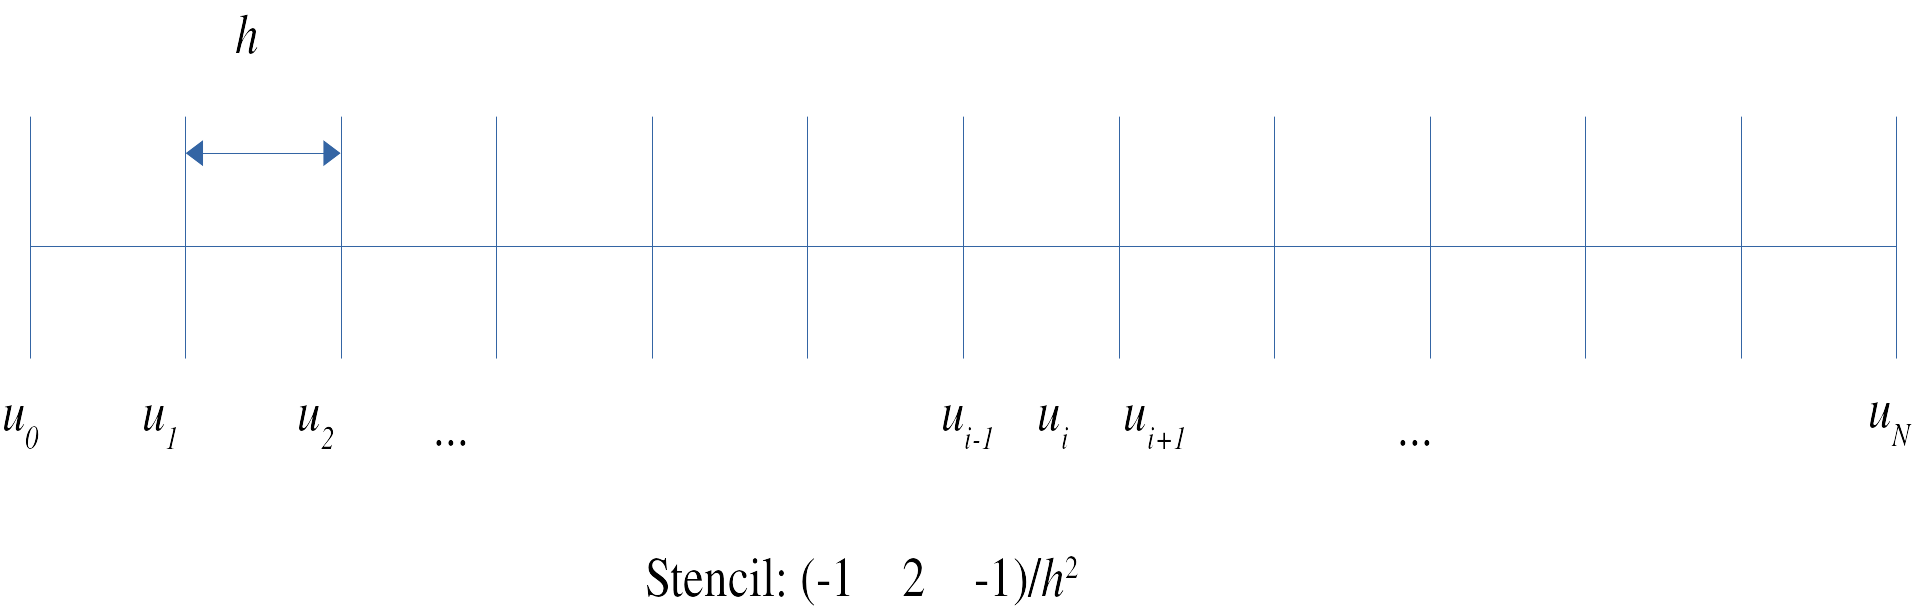
\includegraphics[width=0.7\textwidth]{../figures/1DFDPoisson}
\end{center}
\eq{
\frac{1}{h^2}\begin{bmatrix}
2 & -1 & & & & & & \\
-1 & 2 & -1 & & & & & \\
& -1 & 2 & - 1 & & & & \\
&  & \ddots & \ddots & \ddots & & & \\
& & & & & & & \\
& & & & & -1 & 2 & -1 \\
& & & & & & -1 & 2 \\
\end{bmatrix}
\begin{bmatrix}
u_1 \\
u_2 \\
\\
\vdots \\
\\
\\
u_{N-1} \\
\end{bmatrix}
=
\begin{bmatrix}
f_1 \\
f_2 \\
\\
\vdots \\
\\
\\
f_{N-1} \\
\end{bmatrix}
}
\end{block}
\end{frame}

% Slide
\begin{frame}{Basic iterative methods on a model problem}
\begin{block}{Review of eigenvalues and eigenvectors}
\bit
\item Eigenvalues, $\lambda_k$, and eigenvectors, $\mathbf{v}_k$, of a matrix, $A$, are defined by
\eq{
   A\mathbf{v}_k = \lambda_k \mathbf{v}_k
}
\item Evals and evecs can be a way to think about ``action" of an operator: rotation and scaling
\item Important in many applications from physics and engineering
\eit
\end{block}
\end{frame}

% Slide
\begin{frame}{Basic iterative methods on a model problem}
\begin{block}{Review of eigenvalues and eigenvectors}
\bit
\item If $A$ is symmetric positive definite (SPD), then eigenvalues are real and positive and eigenvectors form an orthonormal basis for $\mathcal{R}^{N-1}$
\item Thus, any vector, $\mathbf{x}\in\mathcal{R}^{N-1}$ can be decomposed as 
\eq{
   \mathbf{x} = \sum_{k=1}^{N-1} \langle \mathbf{x}, \mathbf{v}_k \rangle \mathbf{v}_k 
}
\item We can study behavior of iterative methods by considering their effect on different eigenvectors
\eit
\end{block}
\end{frame}

% Slide
\begin{frame}{Basic iterative methods on a model problem}
\begin{block}{Evals and evecs of the model problem}
\bit
\item $A = tridiag(-1,2,-1)$, then
\eq{
   \lambda_k &= 4\sin^2\left(\frac{k\pi}{2N}\right), &k = 1,...,N-1 \\
   v_k,j &= \sin\left(\frac{jk\pi}{N}\right), &j,k = 1,...,N-1 
}
\eit
\end{block}
\end{frame}

% Slide
\begin{frame}{Basic iterative methods on a model problem}
\begin{block}{Jacobi on the model problem}
\bit
\item Recall the Jacobi iteration
\eq{
   \mathbf{u} \leftarrow D^{-1}(\mathbf{f} + (L+U)\mathbf{u})
}
\item Jacobi is a matrix splitting iteration with error propagation matrix
\eq{
   E &= D^{-1}(L+U) \\
   &= I - D^{-1}A
}
\eit
\end{block}
\end{frame}

% Slide
\begin{frame}{Basic iterative methods on a model problem}
\begin{block}{Jacobi on the model problem}
\bit
\item $E$ and $A$ have the same evecs, $\mathbf{v}_k$
\item The evals, $\tilde\lambda_k$, of $E$ are related to those of $A$ (recall $D = 2I$)
\eq{
   \tilde\lambda_k &= 1 - \frac{1}{2}\lambda_k \\
   &= 1 - 2\sin^2\left(\frac{k\pi}{2N}\right)
}
\eit
\end{block}
\end{frame}


% Slide
\begin{frame}{Basic iterative methods on a model problem}
\begin{block}{Error reduction for Jacobi}
\bit
\item Given initial error, $\mathbf{e}^{(0)}$, error on the $i^th$ iteration is 
\eq{
   \mathbf{e}^{(i)} &= E^i\mathbf{e}^{(0)} \\
   &= E^i\left(\sum_{k=1}^{N-1} \langle \mathbf{e}^{(0)}, \mathbf{v}_k \rangle \mathbf{v}_k\right) \\
   &= \sum_{k=1}^{N-1} \tilde\lambda_k^i \langle \mathbf{e}^{(0)}, \mathbf{v}_k \rangle \mathbf{v}_k
}
\item So the $k^{th}$ ``error mode" is reduced by $\tilde\lambda_k$ on each iteration
\eit
\end{block}
\end{frame}

% Slide
\begin{frame}{Basic iterative methods on a model problem}
\begin{block}{Error reduction for Jacobi}
\bit
\item Error modes associated with large and small evals are damped very slowly
\eq{
   \tilde\lambda_k = 1 - 2\sin^2\left(\frac{k\pi}{2N)}\right)
}
\eit
\end{block}
\begin{center}
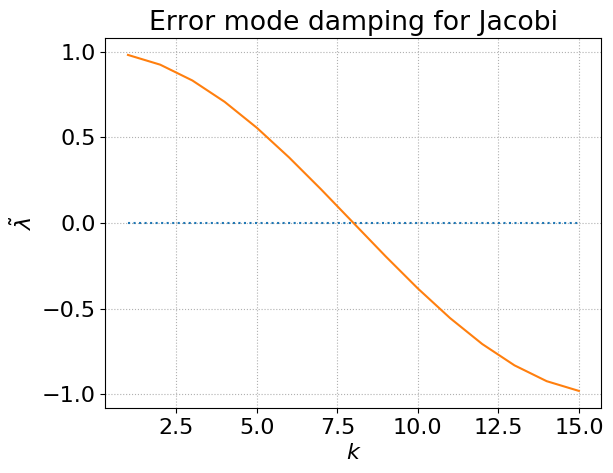
\includegraphics[width=0.5\textwidth]{../figures/jacobiModeDamping}
\end{center}
\end{frame}

% Slide
\begin{frame}{Basic iterative methods on a model problem}
\begin{block}{Weighted Jacobi}
\bit
\item In practice, Jacobi is usually modified with a weighting parameter, $\omega$
\eq{
   \mathbf{u} \leftarrow (1 - \omega)\mathbf{u} + \omega D^{-1}(\mathbf{f} + (L+U)\mathbf{u})
}
\item The error propagation matrix in this case is
\eq{
   E &= I - \omega D^{-1}A
}
\item The associated evals are
\eq{
   \tilde\lambda_k &= 1 - 2\omega\sin^2\left(\frac{k\pi}{2N)}\right)
}
\eit
\end{block}
\end{frame}

% Slide
\begin{frame}{Basic iterative methods on a model problem}
\begin{center}
\begin{block}{Error reduction for Jacobi}
\bit
\item With appropriate $\omega$, can effectively damp modes associated with large $k$
\eq{
   \tilde\lambda_k = 1 - 2\omega\sin^2\left(\frac{k\pi}{2N}\right)
}
\eit
\end{block}
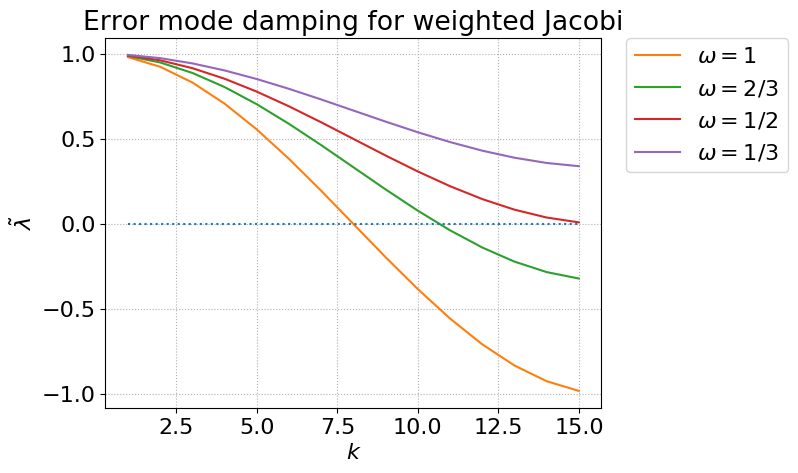
\includegraphics[width=0.6\textwidth]{../figures/weightedJacobiModeDamping}
\end{center}
\end{frame}

% Slide
\begin{frame}{Basic iterative methods on a model problem}
\begin{block}{Gauss-Seidel}
\bit
\item Gauss-Seidel exibits similar behavior
\item Evecs of error propagation, $E$, for Gauss-Seidel are not the same as the evecs of $A$
\item Gauss-Seidel also damps the evecs of $A$ associated with large evals
\eit
\end{block}
\end{frame}

%%%%%%%%%%%%%%%%%%%%%%%%%%%%%%%%%%%%%%%%%%%%%%%%%%%%%%%%%%%%%%%%%%%%%%%%%%%%%%%%

\section{Towards multigrid}

% Slide
\begin{frame}{Towards multigrid}
\begin{block}{Observations}
\bit
\item Weighted Jacobi and Gauss-Seidel are not good solvers on their own
\item They do a good job at damping certain error modes for the model problem
\item Specifically, they remove ``high-frequency" error (they damp the oscillatory evecs of $A$)
\item Call these ``smoothers" or ``relaxation methods"
\eit
\end{block}
\end{frame}

% Slide
\begin{frame}{Towards multigrid}
\begin{block}{Observations}
\bit
\item Smooth modes are representable on a coarser grid
\item Furthermore, they are relatively more oscillatory on that grid 
\eit
\end{block}
\only<1>{
\begin{center}
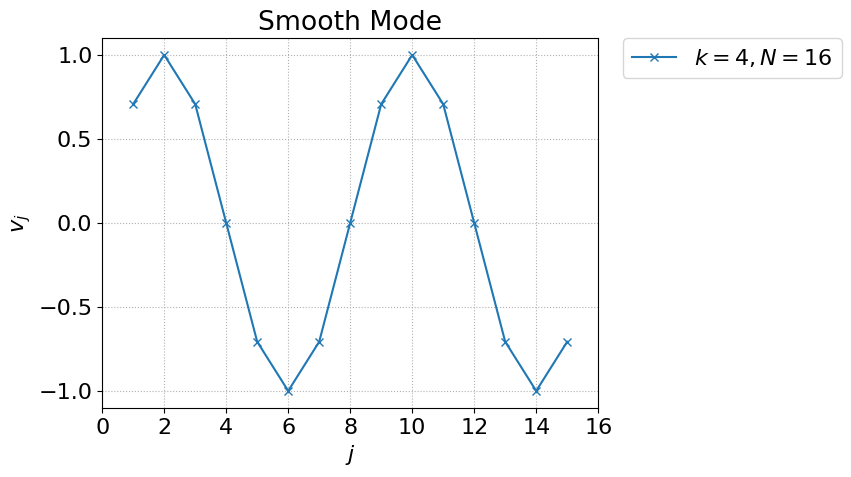
\includegraphics[width=0.6\textwidth]{../figures/smoothMode}
\end{center}
}
\only<2>{
\begin{center}
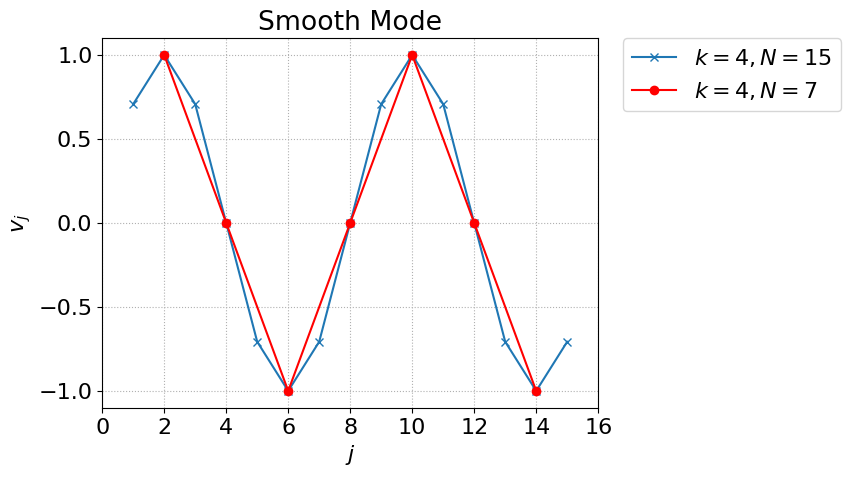
\includegraphics[width=0.6\textwidth]{../figures/modeCoarse}
\end{center}
}
\end{frame}

% Slide
\begin{frame}{Towards multigrid}
\begin{block}{Observations}
\bit
\item Recall that relaxation makes the error, $\mathbf{e}$, smooth (even if the solution, $\mathbf{u}$, is oscillatory)
\item The error satisfies the residual equation
\eq{
   A\mathbf{e} = \mathbf{r}
}
\item Idea: can use relaxation on a coarse grid to effectively solve the residual equation! 
\eit
\end{block}
\end{frame}

% Slide
\begin{frame}{Towards multigrid}
\begin{block}{Coarse-grid correction}
\bit
\item Relax on $A\mathbf{u} = \mathbf{f}$ to obtain approximate solution, $\mathbf{u}$
\item Error, $\mathbf{e} = \mathbf{\tilde u} - \mathbf{u}$, is smooth
\item Calculate the residual $\mathbf{r} = \mathbf{f} - A\mathbf{u}$
\item Relax on $A\mathbf{e} = \mathbf{r}$ on a coarse grid to obtain approximate correction, $\mathbf{e}$
\item Correct on the fine grid $\mathbf{u} \leftarrow \mathbf{u} + \mathbf{e}$
\eit
\end{block}
\end{frame}

% Slide
\begin{frame}{Towards multigrid}
\begin{block}{Remaining questions}
\bit
\item How to define the coarse grid?
\item How to move between grid levels?
\item How to go from two-grid to multigrid?
\eit
\end{block}
\end{frame}

%%%%%%%%%%%%%%%%%%%%%%%%%%%%%%%%%%%%%%%%%%%%%%%%%%%%%%%%%%%%%%%%%%%%%%%%%%%%%%%%

\section{Components of multigrid}

% Slide
\begin{frame}{Components of multigrid}
\begin{block}{Components of multigrid}
\bit
\item Hierarchy of grids and associated problems
\item Relaxation methods to apply to problems on each grid level
\item Interpolation from coarse to fine grids
\item Restriction from fine to coarse grids
\item Cycle structure
\eit
\end{block}
\end{frame}

% Slide
\begin{frame}{Components of multigrid}
\begin{block}{Coarse grids}
\bit
\item Rediscretize the PDE with half the step size
\eit
TODO Figure
\end{block}
\end{frame}

% Slide
\begin{frame}{Components of multigrid}
\begin{block}{Interpolation (prolongation)}
\bit
\item Linear interpolation
\item Identity at C-points
\item Average of neighbors at F-points
\eq{
   e^f_i = \begin{cases}
   e^c_{i/2}, &i \,\,\text{even} \\
   \frac{1}{2}(e^c_{(i-1)/2} + e^c_{(i+1)/2}, &i \,\,\text{odd}
   \end{cases}
}
\eit
\end{block}
\end{frame}

% Slide
\begin{frame}{Components of multigrid}
\begin{block}{}
\bit
\item 
\eit
\end{block}
\begin{center}
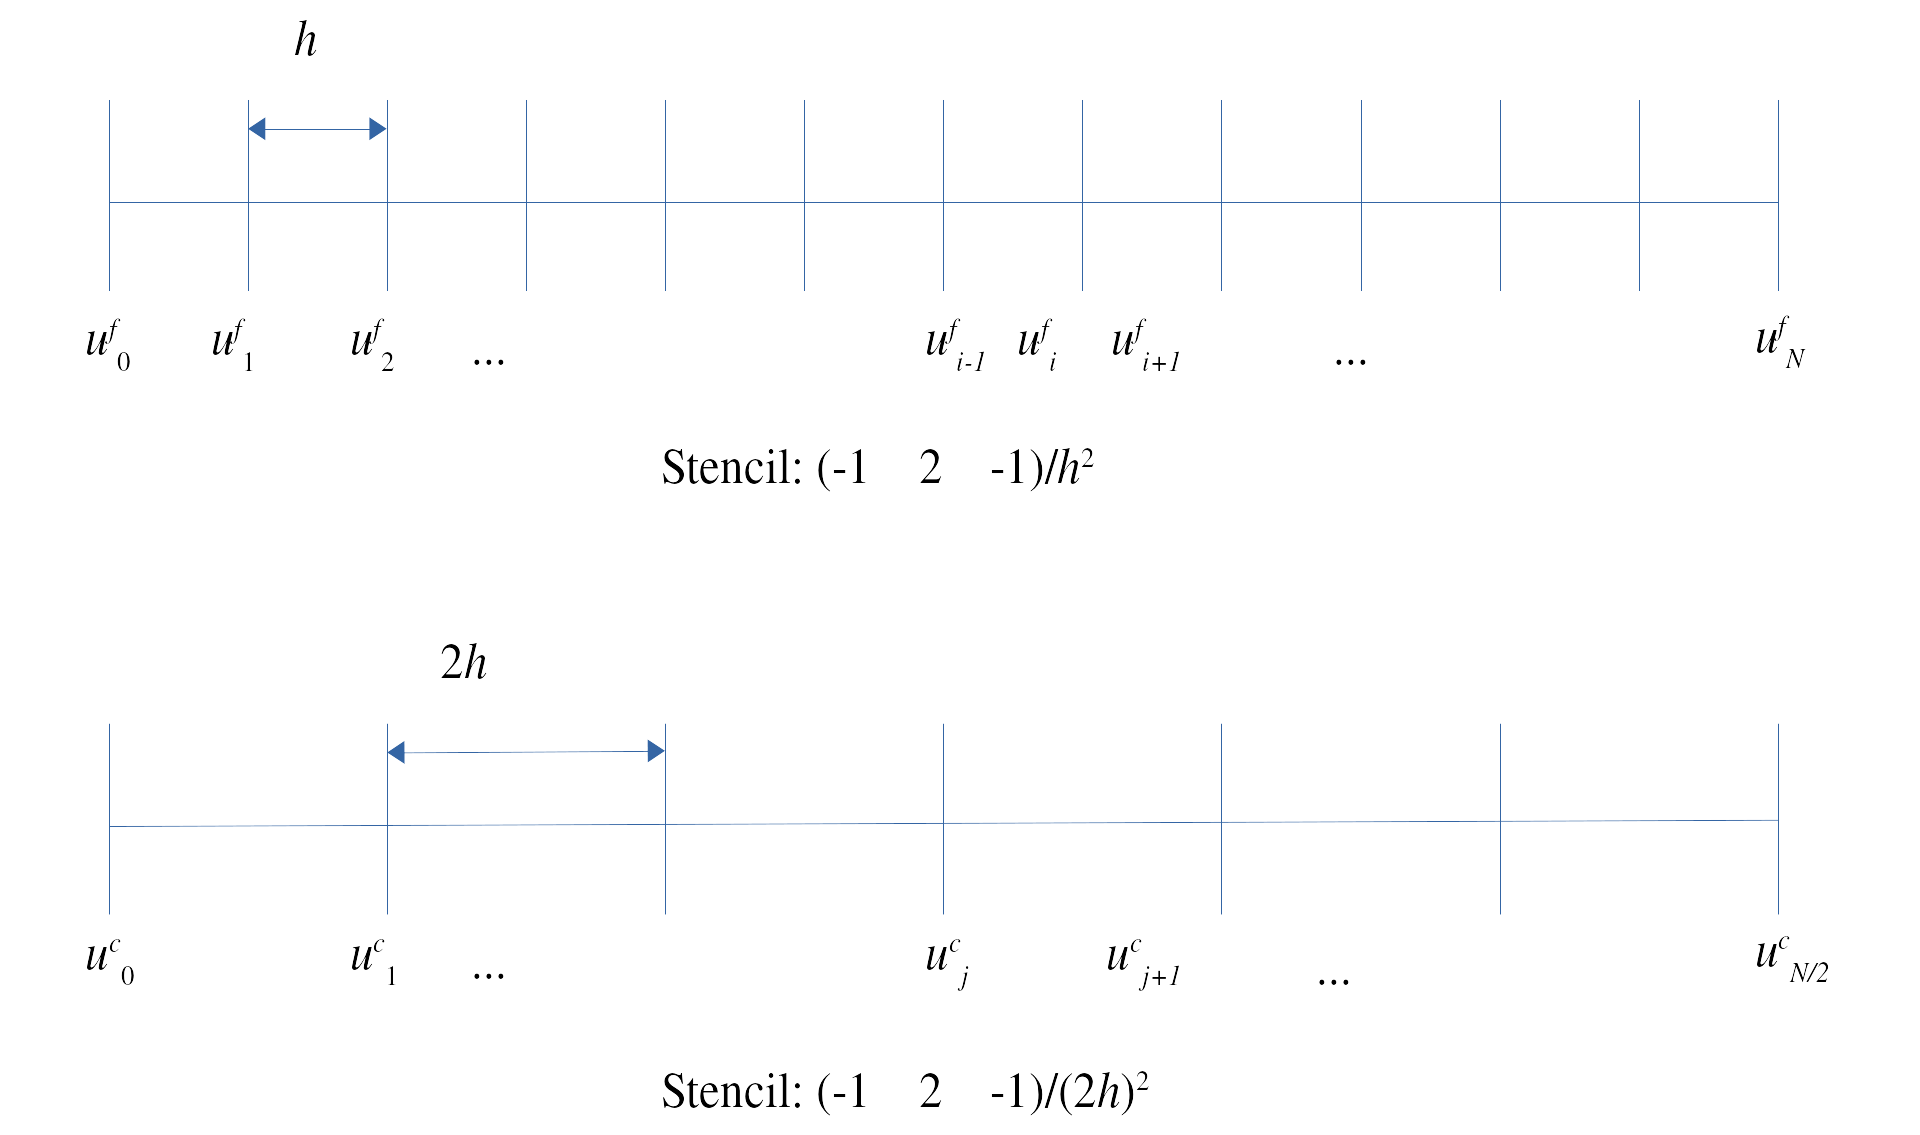
\includegraphics[width=0.7\textwidth]{../figures/coarse1DFDPoisson}
\end{center}
\end{frame}

% Slide
\begin{frame}{Components of multigrid}
\begin{block}{}
\bit
\item 
\eit
\end{block}
\begin{center}
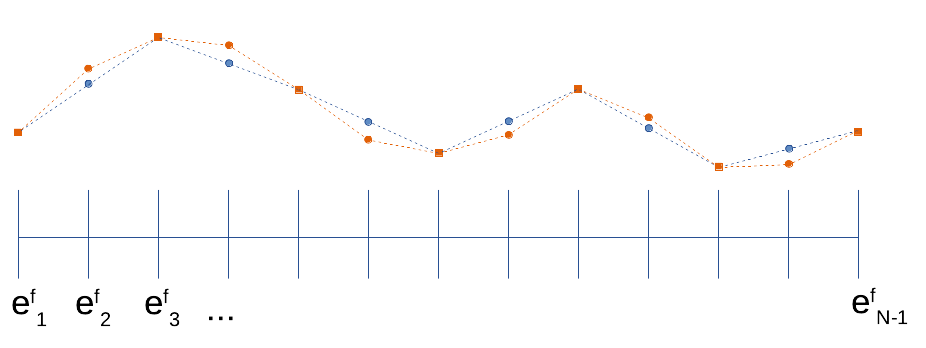
\includegraphics[width=0.7\textwidth]{../figures/coarseCorrectionSmooth}
\end{center}
\end{frame}

% Slide
\begin{frame}{Components of multigrid}
\begin{block}{}
\bit
\item 
\eit
\end{block}
\begin{center}
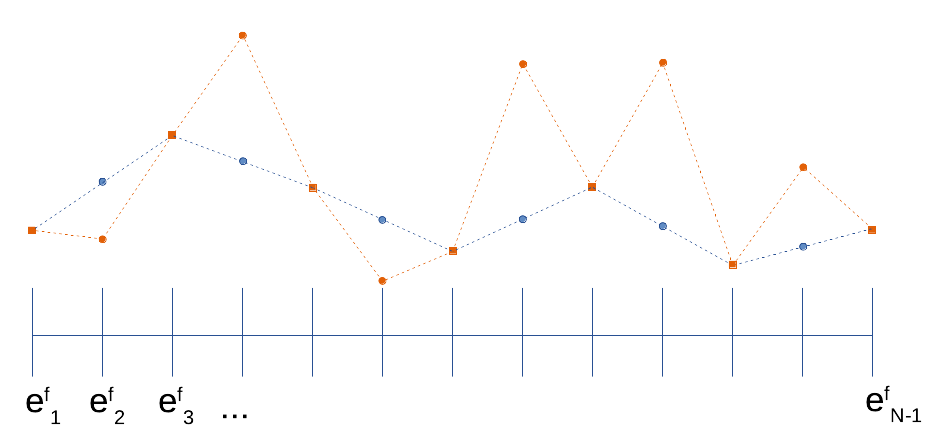
\includegraphics[width=0.7\textwidth]{../figures/coarseCorrectionOscillatory}
\end{center}
\end{frame}

% Slide
\begin{frame}{Components of multigrid}
\begin{block}{}
\bit
\item 
\eit
\end{block}
\begin{center}
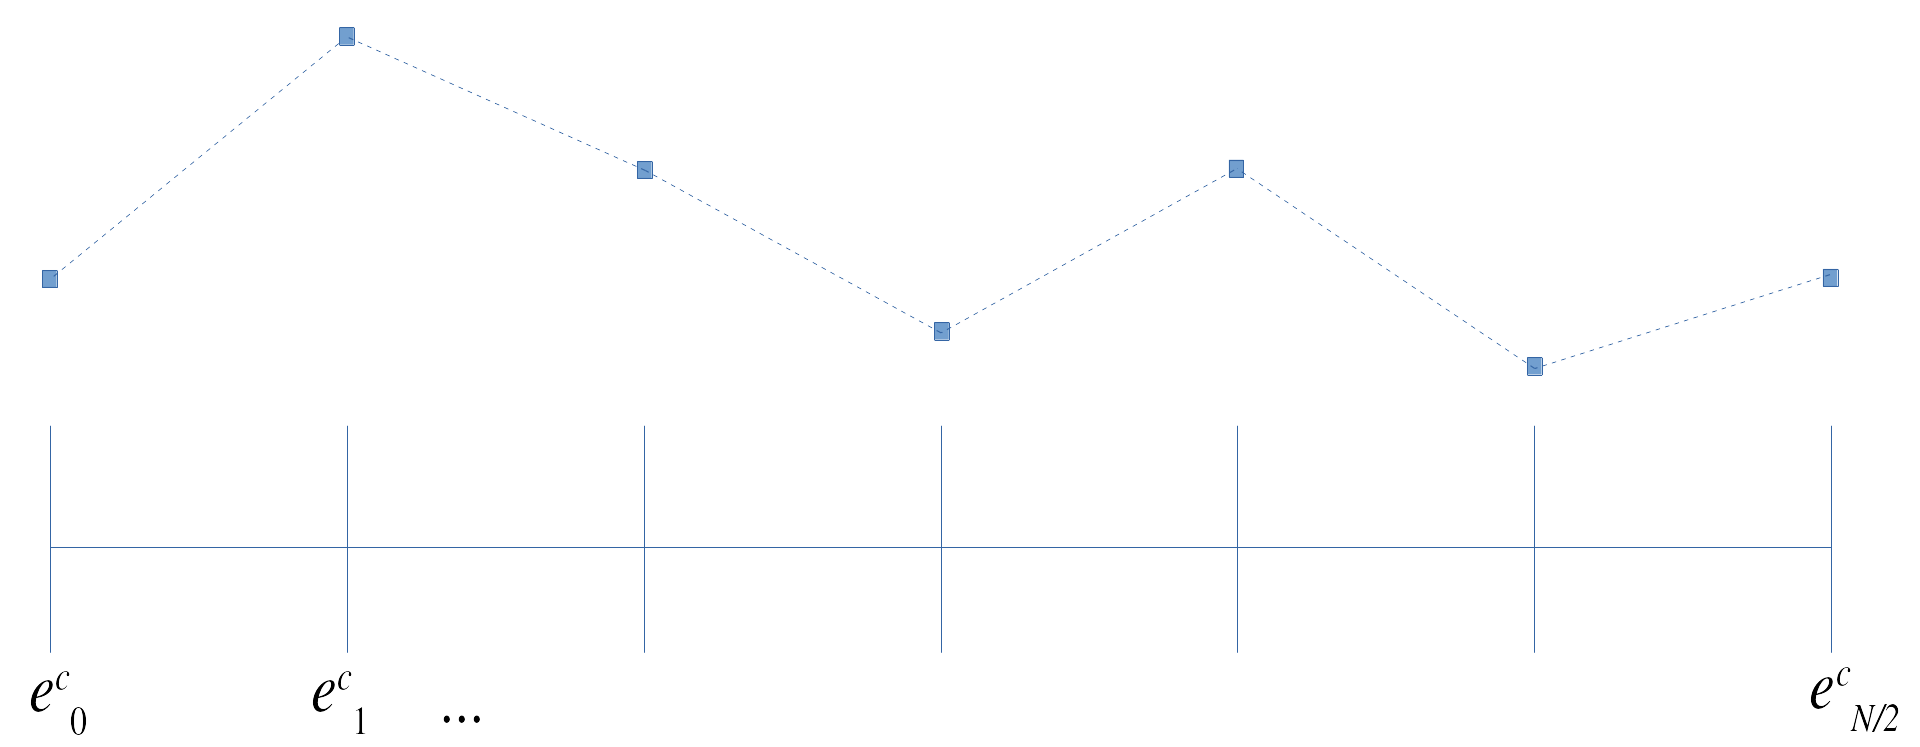
\includegraphics[width=0.7\textwidth]{../figures/coarseError}
\end{center}
\end{frame}

% Slide
\begin{frame}{Components of multigrid}
\begin{block}{}
\bit
\item 
\eit
\end{block}
\begin{center}
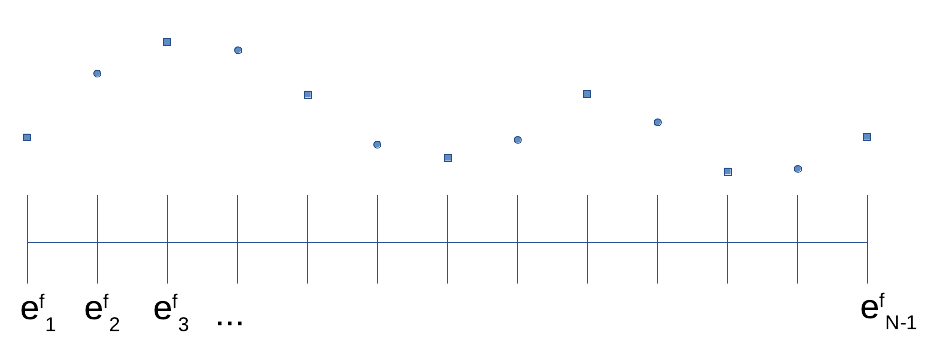
\includegraphics[width=0.7\textwidth]{../figures/fineResidual}
\end{center}
\end{frame}

% Slide
\begin{frame}{Components of multigrid}
\begin{block}{}
\bit
\item 
\eit
\end{block}
\begin{center}
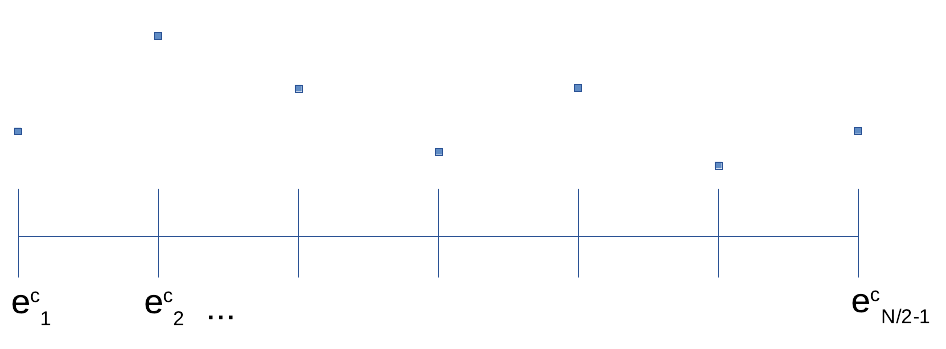
\includegraphics[width=0.7\textwidth]{../figures/injectedResidual}
\end{center}
\end{frame}

% Slide
\begin{frame}{Components of multigrid}
\begin{block}{}
\bit
\item 
\eit
\end{block}
\begin{center}
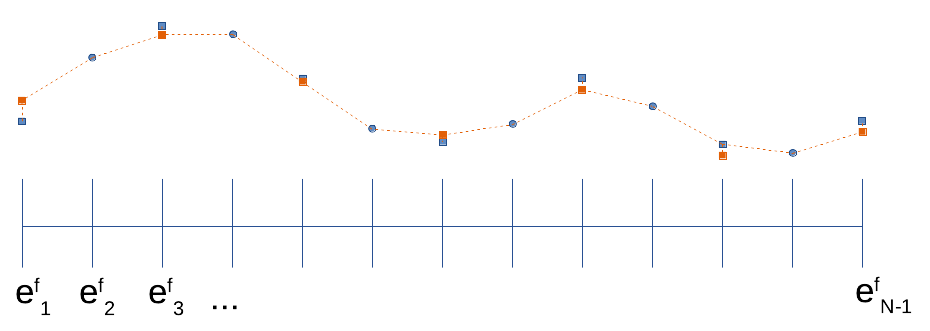
\includegraphics[width=0.7\textwidth]{../figures/fullWeightingResidual}
\end{center}
\end{frame}

% Slide
\begin{frame}{Components of multigrid}
\begin{block}{}
\bit
\item 
\eit
\end{block}
\end{frame}

% Slide
\begin{frame}{Components of multigrid}
\begin{block}{}
\bit
\item 
\eit
\end{block}
\end{frame}


% Define coarse grids
% Define relaxation
% Define interpolation
% Define restriction
% Define 2 grid
% Define MG cycles
% Cost of MG: count up the operations to get compute cost

%%%%%%%%%%%%%%%%%%%%%%%%%%%%%%%%%%%%%%%%%%%%%%%%%%%%%%%%%%%%%%%%%%%%%%%%%%%%%%%%

\section{Some basic convergence theory}

% Slide
\begin{frame}{Some basic convergence theory}
\begin{block}{}
\bit
\item
\eit
\end{block}
\end{frame}

% Two grid convergence
% multilevel?
% FMG convergence to discretization accuracy

%%%%%%%%%%%%%%%%%%%%%%%%%%%%%%%%%%%%%%%%%%%%%%%%%%%%%%%%%%%%%%%%%%%%%%%%%%%%%%%%

\section{Other stuff?}

% Generally mention that we've developed all this stuff for Poisson, but you can do similar stuff for more general problems: Just have to figure out how to construct effective MG components for your problem. Forshadow AMG tries to do this as a black box.
% 2D examples, anisotropic examples with line smoothing and semicoarsening
% Use of MG as preconditioner for Krylov methods


%%%%%%%%%%%%%%%%%%%%%%%%%%%%%%%%%%%%%%%%%%%%%%%%%%%%%%%%%%%%%%%%%%%%%%%%%%%%%%%%


% Slide
\begin{frame}{}
\begin{block}{}
\bit
\item 
\eit
\end{block}
\end{frame}



%%%%%%%%%%%%%%%%%%%%%%%%%%%%%%%%%%%%%%%%%%%%%%%%%%%%%%%%%%%%%%%%%%%%%%%%%%%%%%%%

\end{document}

